\documentclass[a4paper]{article}    % define document layout
%\documentclass[draft]{article}     % use draft option in packages
%-----------------------------
% preamble
%-----------------------------
\usepackage[sumlimits,]{amsmath}    % math equations and formulas
\usepackage[utf8]{inputenc}         % use UTF-8 encoding
\usepackage[english]{babel}         % use English language
\usepackage{graphicx}              % insert images
%\usepackage[draft]{graphicx}        % do not render figures
\usepackage{subcaption}             % multiple images in one figure
\usepackage{hyperref}               % hyperlinks
\usepackage{float}                  % floating objects (figures, tables)
\usepackage{geometry}               % page size and margins
\geometry{a4paper, margin=1in}      % margins
\usepackage{ragged2e}               % text alignment
\usepackage[table]{xcolor}          % change cell color in tables
%\usepackage{multirow}               % merge rows in table
%\usepackage[thinc]{esdiff}          % macros for derivatives

% MATLAB code
\usepackage{listings}
\usepackage{color} %red, green, blue, yellow, cyan, magenta, black, white
\usepackage{xcolor}

\graphicspath{                      % path for figures
    {../figures/} 
    {../figures/Q8/} 
}

\definecolor{Gray}{gray}{0.8}
\definecolor{codegreen}{rgb}{0,0.6,0}
\definecolor{codegray}{rgb}{0.5,0.5,0.5}
\definecolor{codepurple}{rgb}{0.58,0,0.82}
\definecolor{backcolour}{rgb}{0.95,0.95,0.92}

\lstdefinestyle{mystyle}{
    backgroundcolor=\color{backcolour},   
    commentstyle=\color{codegreen},
    keywordstyle=\color{magenta},
    numberstyle=\tiny\color{codegray},
    stringstyle=\color{codepurple},
    basicstyle=\ttfamily\footnotesize,
    breakatwhitespace=false,         
    breaklines=true,                 
    captionpos=b,                    
    keepspaces=true,                 
    numbers=left,                    
    numbersep=5pt,                  
    showspaces=false,                
    showstringspaces=false,
    showtabs=false,                  
    tabsize=2
}
\lstset{style=mystyle}

%-----------------------------
% body
%-----------------------------
\begin{document}

\begin{figure}
    \centering
    % UNICAMP logo
    \begin{subfigure}{0.45\textwidth}
        \centering
        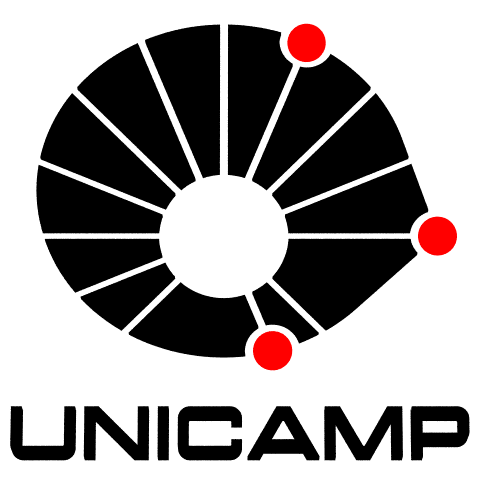
\includegraphics[width=1.5cm]{unicamp}
%        \label{fig:unicamp}
    \end{subfigure}
    \hfill
    % FEEC logo
    \begin{subfigure}{0.45\textwidth}
        \centering
        
\includegraphics[width=1.5cm]{feec}
%        \label{fig:feec}
    \end{subfigure}
\end{figure}

\title{
    \vspace{5cm}
    IA353A - Neural Networks\\
    EFC4
    \vspace{1cm}
}
\author{
    Rafael Claro Ito\\
    (R.A.: 118430)
    \vspace{11cm}
}
%R.A.: 118430
%ito.rafael@gmail.com
\date{July 2020}
\maketitle
\newpage

%=================================================
\section*{Question 8: RL}
%=================================================
\addtocounter{section}{8}

\href{https://drive.google.com/file/d/1Xya6E4BgNVOPlzPRKbb3C59rvKI6V2nk/view?usp=sharing}{https://drive.google.com/file/d/1Xya6E4BgNVOPlzPRKbb3C59rvKI6V2nk/view?usp=sharing}

%------------------------
\subsection{Training results and two study cases}
%------------------------

Maze 1:

\begin{table}[H]
    \begin{center}
        \begin{tabular}{|c|c|c|c|c|c|}
            \cline{1-6}
            \rowcolor{Gray}
            Epoch & Loss & Episodes & Win count & Win rate & Time s \\
            \cline{1-6}
             0 & 0.0317 &  51 &  1 & 0.000 &   2.7 \\
            10 & 0.0766 & 109 &  5 & 0.000 &  45.6 \\
            20 & 0.0023 & 102 & 10 & 0.000 &  77.8 \\
            30 & 0.0012 &   6 & 17 & 0.625 &  97.6 \\
            40 & 0.0627 & 103 & 24 & 0.667 & 117.0 \\
            50 & 0.0010 &   6 & 30 & 0.708 & 143.0 \\
            60 & 0.0025 &   4 & 39 & 0.708 & 152.4 \\
            70 & 0.0065 & 102 & 46 & 0.750 & 176.5 \\
            80 & 0.0019 &   2 & 56 & 0.833 & 188.0 \\
            90 & 0.0013 &  23 & 66 & 0.958 & 198.4 \\
            94 & 0.0010 &  21 & 70 & 1.000 & 199.8 \\
            \cline{1-6}
        \end{tabular}
    \end{center}
    \caption{Training results summary for maze 1}
    \label{tab:maze1-results}
\end{table}


%Reached 100% win rate at epoch: 94
%files: model.h5, model.json
%n_epoch: 94, max_mem: 392, data: 32, time: 200.1 seconds
%200.067352

Maze 2:

\begin{table}[H]
    \begin{center}
        \begin{tabular}{|c|c|c|c|c|c|}
            \cline{1-6}
            \rowcolor{Gray}
            Epoch & Loss & Episodes & Win count & Win rate & Time s \\
            \cline{1-6}
            000 & 0.0856 & 147 &   1 & 0.000 &   8.8 s  \\
            010 & 0.0011 & 219 &   4 & 0.000 & 128.4 s  \\
            020 & 0.0042 &  55 &   6 & 0.000 & 237.7 s  \\
            030 & 0.0041 &  21 &  13 & 0.000 & 297.6 s  \\
            040 & 0.0044 &  67 &  22 & 0.000 & 346.0 s  \\
            050 & 0.0026 &  30 &  31 & 0.600 & 380.5 s  \\
            060 & 0.0043 &  23 &  41 & 0.740 & 6.69 min \\
            070 & 0.0006 &  18 &  51 & 0.900 & 7.00 min \\
            080 & 0.0071 &  35 &  61 & 0.960 & 7.44 min \\
            090 & 0.0005 &  18 &  71 & 0.980 & 7.67 min \\
            100 & 0.0015 &   4 &  81 & 1.000 & 7.92 min \\
            110 & 0.0010 &  11 &  91 & 1.000 & 8.16 min \\
            120 & 0.0008 &  18 & 101 & 1.000 & 8.43 min \\
            130 & 0.0004 &  19 & 111 & 1.000 & 8.84 min \\
            140 & 0.0012 &  20 & 121 & 1.000 & 9.13 min \\
            150 & 0.0007 &  34 & 131 & 1.000 & 9.54 min \\
            160 & 0.0013 &  61 & 141 & 1.000 & 9.83 min \\
            165 & 0.0002 &  28 & 146 & 1.000 & 9.99 min \\
            \cline{1-6}
        \end{tabular}
    \end{center}
    \caption{Training results summary for maze 2}
    \label{tab:maze2-results}
\end{table}

%Reached 100% win rate at epoch: 165
%files: model.h5, model.json
%n_epoch: 165, max_mem: 800, data: 32, time: 10.01 minutes
%600.636667

%------------------------
\subsection{Q-value for three different states}
%------------------------

%------------------------
\subsection{RMS during the training}
%------------------------

%------------------------
\subsection{Experience replay}
%------------------------

%=================================================
\section{Question 9: GAN}
%=================================================

\href{https://drive.google.com/file/d/1WWdc3M0UObMp1jVCcndmor6BTdLe18\_e/view?usp=sharing}{https://drive.google.com/file/d/1WWdc3M0UObMp1jVCcndmor6BTdLe18\_e/view?usp=sharing}

%------------------------
\subsection{MNIST}
%------------------------

%------------------------
\subsection{CIFAR-100 (class: oak tree)}
%------------------------

%=================================================
\section{Question 10: NLP}
%=================================================

\href{https://drive.google.com/file/d/1EAU2toNRn-MjXyO_YAsZFejdaJDapibX/view?usp=sharing}{https://drive.google.com/file/d/1EAU2toNRn-MjXyO\_YAsZFejdaJDapibX/view?usp=sharing}

%------------------------
\subsection{Word2Vec}
%------------------------

%------------------------
\subsection{t-SNE}
%------------------------

%------------------------
\subsection{Results discussion}
%------------------------

%=================================================

\end{document}
